\section{Einführung}

\begin{bonus}{Web 2.0}
    Von passiver \enquote{Informations}-Nutzung zur aktiven Nutzung.
    
    Neben der ursprünglich unidirektionalen Kommunikation von Servern zu Clients, werden nun ebenfalls Daten von Clients an Server gesendet.
    Diese sind z. B. Inhalte in Foren, Podcasts, YouTube-Videos etc.
    %Hinzu kommen noch Webanwendungen wie Microsoft Office 365, Google Drive, Discord, draw.io etc.
    
    Das ursprüngliche Web bestand aus:
    \begin{itemize}
        \item Dokumenten (HTML), die eindeutig adressiert (URL) werden können und sich untereinander referenzieren.
        \item einem festen Übertragungsprotokoll (HTTP)
        \item Servern, die diese Dokumente bereit stellen.
        \item Clients (Browser), die Anfragen des Benutzenden an Server übertragen und dessen Antwort aufbereiten.
    \end{itemize}
    
    \begin{center}
        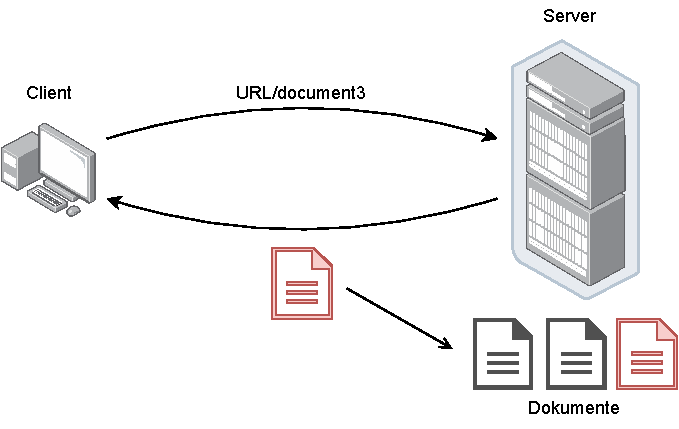
\includegraphics[width=0.5\textwidth]{includes/figures/bonus_original_web.pdf}
    \end{center}
\end{bonus}

\begin{defi}{Webserver}
    \emph{Webserver} sind Dienste, die Anfragen von Clients bearbeiten.
    
    Diese Anfragen werden von einer oder mehreren \emph{Webserver-Software} Anwendungen bearbeitet.
    Vorreiter dieser Anwendungen sind \emph{Nginx} (33.1\%) und \emph{Apache} (30.8\%).
    
    Die Verzeichnisstruktur und damit insbesondere auch das Einstiegsverzeichnis (gelb) ist dabei abhängig von dem Betriebssystem bzw. der Distribution:
    
    \begin{minipage}[t]{.5\textwidth}
        XAMPP (Windows):
        
        \centering
        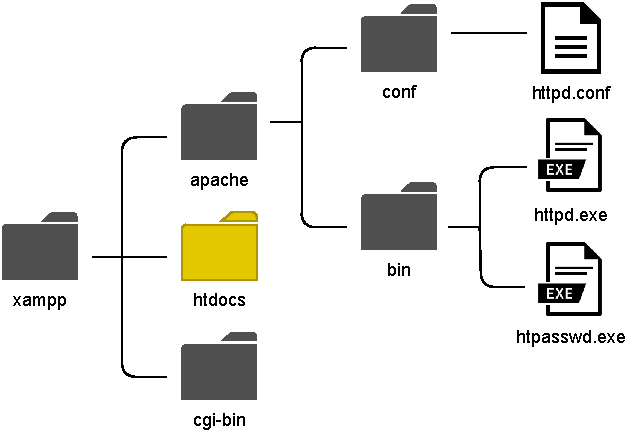
\includegraphics[width=.9\textwidth]{includes/figures/defi_xampp.pdf}
    \end{minipage}%
    \begin{minipage}[t]{.5\textwidth}
        Apache (Ubuntu):
        
        \centering
        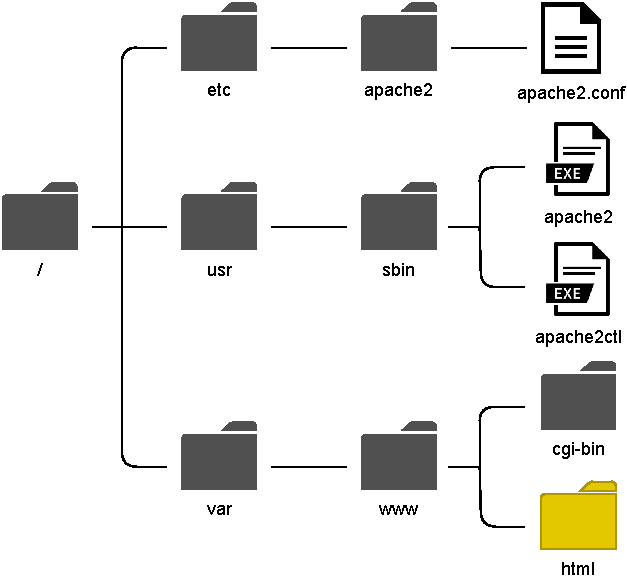
\includegraphics[width=.9\textwidth]{includes/figures/defi_apache.pdf}
    \end{minipage}
\end{defi}

\begin{bonus}{XAMPP}
    \emph{XAMPP} ist ein Akronym und steht für: 
    \begin{itemize}
        \item X: Plattformunabhängigkeit,
        \item A: Apache (HTTP-Server),
        \item M: MariaDB,
        \item P: PHP
        \item P: Perl
    \end{itemize}
    
    Viele Konfigurationen sind in Produktiveinsätzen unsicher, z. B. wird ein auftretender PHP-Error dem Nutzenden angezeigt.
    Ebenfalls sind alle Verzeichnisinhalte zugänglich.
    
    Des Weiteren bietet XAMPP nur eingeschränkte (Rolling-)Update- und Clustermöglichkeiten.
    
    XAMPP ist ausschließlich als Entwicklungssystem geeignet.
    
    % Als Produktivsystem findet man meistens Ubuntu, Debian, Red Hat oder einen Docker Container.
\end{bonus}